% Histogram [2, 1, 4, 5, 1, 3, 3]; hatching marks the maximum rectangle (width 2, height 4).
% Editable source for this diagram. From this directory, regenerate with:
% latex -interaction=nonstopmode -halt-on-error cartesian-tree-3.tex
% dvisvgm --no-fonts --exact --bbox=papersize --output=cartesian-tree-3.svg cartesian-tree-3.dvi
\documentclass[tikz,border=2pt]{standalone}
\usepackage{lmodern}
\usepackage{tikz}
\usetikzlibrary{arrows.meta,backgrounds,shapes.geometric,patterns}
\definecolor{linkred}{HTML}{B5240A}
\definecolor{noteBlue}{HTML}{0067A5}
\definecolor{softgreen}{HTML}{D8EAD0}
\definecolor{softpurple}{HTML}{D9D1E8}
\definecolor{softpink}{HTML}{F5CECF}
\definecolor{softyellow}{HTML}{FFF2C9}
\begin{document}
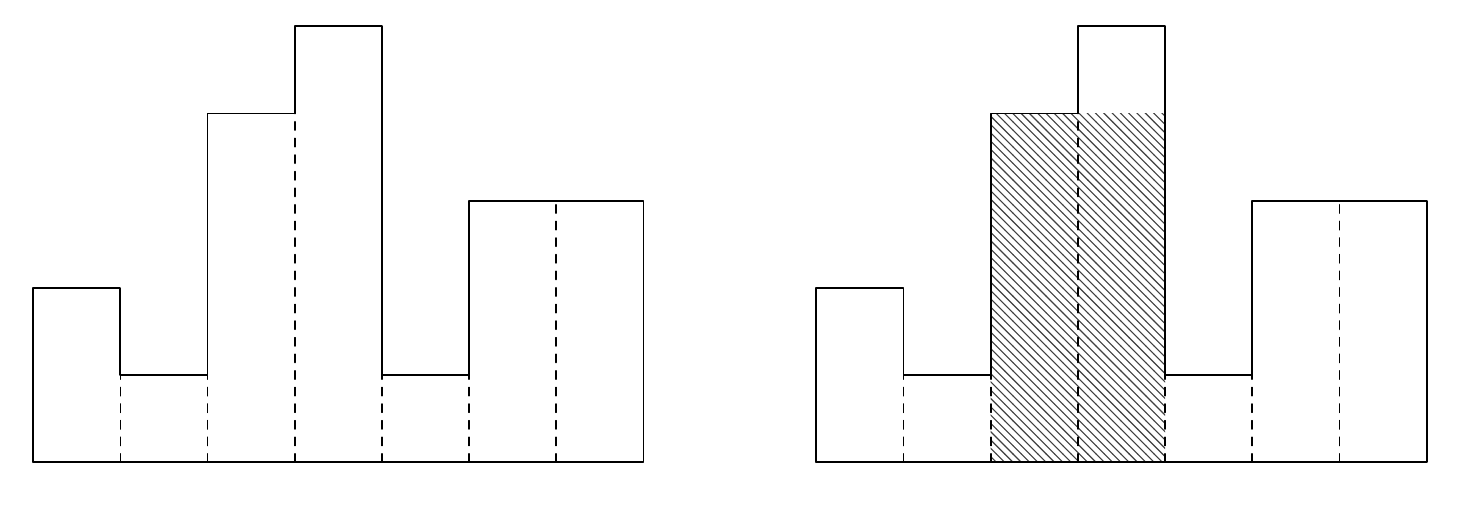
\begin{tikzpicture}[x=1pt,y=-1pt,>=Stealth,line cap=round,line join=round]
\path[use as bounding box] (0,0) rectangle (510,165);
\begin{scope}[on background layer]
\fill[pattern=north west lines,pattern color=black!75] (348.0,31) rectangle (411.0,157);
\end{scope}

\begin{scope}[on background layer]

\end{scope}
\draw[draw=black,line width=0.65pt] (2,157) -- (2,94.0) -- (33.5,94.0) -- (33.5,125.5) -- (65.0,125.5) -- (65.0,31.0) -- (96.5,31.0) -- (96.5,-0.5) -- (128.0,-0.5) -- (128.0,125.5) -- (159.5,125.5) -- (159.5,62.5) -- (191.0,62.5) -- (191.0,62.5) -- (222.5,62.5) -- (222.5,157) -- (2,157);
\draw[draw=black,line width=0.6pt,dashed] (33.5,157) -- (33.5,125.5);
\draw[draw=black,line width=0.6pt,dashed] (65.0,157) -- (65.0,125.5);
\draw[draw=black,line width=0.6pt,dashed] (96.5,157) -- (96.5,31.0);
\draw[draw=black,line width=0.6pt,dashed] (128.0,157) -- (128.0,125.5);
\draw[draw=black,line width=0.6pt,dashed] (159.5,157) -- (159.5,125.5);
\draw[draw=black,line width=0.6pt,dashed] (191.0,157) -- (191.0,62.5);
\draw[draw=black,line width=0.65pt] (285,157) -- (285,94.0) -- (316.5,94.0) -- (316.5,125.5) -- (348.0,125.5) -- (348.0,31.0) -- (379.5,31.0) -- (379.5,-0.5) -- (411.0,-0.5) -- (411.0,125.5) -- (442.5,125.5) -- (442.5,62.5) -- (474.0,62.5) -- (474.0,62.5) -- (505.5,62.5) -- (505.5,157) -- (285,157);
\draw[draw=black,line width=0.6pt,dashed] (316.5,157) -- (316.5,125.5);
\draw[draw=black,line width=0.6pt,dashed] (348.0,157) -- (348.0,125.5);
\draw[draw=black,line width=0.6pt,dashed] (379.5,157) -- (379.5,31.0);
\draw[draw=black,line width=0.6pt,dashed] (411.0,157) -- (411.0,125.5);
\draw[draw=black,line width=0.6pt,dashed] (442.5,157) -- (442.5,125.5);
\draw[draw=black,line width=0.6pt,dashed] (474.0,157) -- (474.0,62.5);
\end{tikzpicture}
\end{document}
